\chapter{Objektorientierte Analyse}


\section{Lernziele}

\begin{itemize}
    \item für kleinere Projekte qualitätssichernde Maßnahmen planen und verfolgen können
    \item Tests planen und dokumentieren können
    \item gefundene Fehler geeignet verwalten können
\end{itemize}

\newpage


\section{Modelle in Analyse und Entwurf}

\subsection*{Analyse}

\vspace{2mm}
Die Analyse beschreibt fachliche Zusammenhänge, keine technischen.
\vspace{2mm}



Bereits in der ersten Phase der Softwareentwicklung gesammelte Anforderungen können nicht direkt umgesetzt werden, da sie meist viel zu ungenau sind.
Offene Punkte müßten durch einen dauernden Kontakt zu Endanwender und Kunde geklärt werden.\\
Außerdem zeigt sich, dass Anforderungen in sich widersprüchlich sein können, ohne, dass das auf den ersten Blick erkennbar ist.\\

\noindent
Eine Lösung wäre es, die Dokumente aus der Anforderungsphase sehr formal zu gestalten, wodurch die Dokumente aber sehr umfangreich und schwer verständlich werden.\\

\noindent
Stattdessen erstellt man in der \textbf{Analysephase} ein formales Modell sowohl des Problems \textit{in seinem Umfeld} als auch der Lösung.

\subsection*{Entwurf}
In der \textbf{Entwurfsphase} werden die \textbf{Architektur} der Anwendung bestimmt, unter Berücksichtung technischer Randbedingungen, die im Rahmen nicht-funktionaler Anforderungen in der Anforderungsphase gesammelt wurden und vom Kunden stammen (s. Abschnitt~\ref{subsec:technische-randbedingung}).\\
Die Architektur schließt u.a. ein:

\begin{itemize}
    \item Programmiersprache
    \item Frameworks
    \item Einsatz von Datenbanken
    \item \ldots
\end{itemize}

\noindent
Meist bleiben im Anschluss technische Fragen offen, die in der \textbf{Entwurfsphase} beantwortet werden.

\begin{itemize}
    \item Welche \textbf{Klassen} aus der \textbf{Analyse} können übernommen werden?
    \item Wie werden Klassen in einem relationalen Datenbank-Schema gespeichert?
    \item Welche Steuerungklassen müssen für die GUI implementiert werden?
\end{itemize}

\noindent
Das Erstellen eines Modells der geplanten Software bietet den Vorteil, das Entwurfs-Alternativen einfacher und schneller durchdacht werden können, und die Zusammenarbeit einfacher ist, wenn die Umsetzung genauer geplant wird (vgl. \cite[2]{Wed09b}).


\subsection*{Definition Modell}


\vspace{2mm}
\begin{tcolorbox}[title=Arbeitsdefinition ``Modell``]
    Ein \textbf{Modell} ist ein Produkt des \textbf{Modellierungsvorgangs}.\\

    \noindent
    Es beschriebt tatsächliche oder gedachte Gegenstände oder Konzepte und deren Beziehungen.\\

    \noindent
    Ein Modell erfasst diese Konzepte nicht vollständig, sondern \textbf{abstrakt}, also verkürzt und vereinfacht (vgl. \cite[2]{Wed09b}).
\end{tcolorbox}
\vspace{2mm}

\subsection*{Statische und dynamische Modelle}

\noindent
Modelle der Analyse und des Entwurfs bestehen aus miteinander verzahnten \textbf{statischen} und \textbf{dynamischen} Modellen:

\begin{itemize}
    \item \textbf{statische Modelle} beschreiben die Bausteine eines Systems und wie sie zusammengesetzt sind\footnote{vergleichbar mit technischen Zeichnungen}
    \item \textbf{dynamische Modelle} beschreiben die Zusammenarbeit der Bausteine, also deren verhalten und die Nachrichten, die Verhalten auslösen
\end{itemize}

\noindent
\textbf{Dynamische Modelle} sind \textit{notwendig}, da das Zusammenspiel der Modellelemente aus dem statischen Modell nicht immer eindeutig abgeleitet werden kann.\\

\noindent
Als Grundlage zur Modellierung wird meist der \textbf{objektorientierte} Ansatz gewählt\footnote{
    mit dem Vorteil, dass für die Modellierung dieselben Techniken gewählt werden wie bei der späteren Umsetzung
}.\\

\noindent
Hierfür wird i.d.R. \textbf{UML}\footnote{
s. UML Version 2.5.1: \url{https://www.omg.org/spec/UML/}, abgerufen 10.04.2024
} verwendet, damit die Beschreibung eindeutig für alle Benutzer ist.
\section{Klassen und Objekte}

\noindent
\textbf{Klassen} sind Abstraktionen von Objekten.\\

\noindent
\textbf{Objekte} besitzen Eigenschaften und Verhalten.\\

\noindent
In der \textbf{UML} werden Attribute und Verantwortlichkeiten oder Operationen in \textbf{Compartments} (dt. \textit{Abteilungen}) dargestellt.\\

\noindent
Einschränken des Typs können hinter dem Typ in geschweiften Klammern in der \textbf{Object Constraint Language}-Notation\footnote{
s. Version 2.4: \url{https://www.omg.org/spec/OCL}, abgerufen 11.04.2024
} (\textbf{OCL}) angegeben werden\footnote{
alternativ können Kommentare in entsprecheder UML-Notation angegeben werden.
}
Diese Angaben - oder als Kommentar in Textform angegeben - ersetzen im \textit{Klassendiagramm der Analyse} das \textbf{Datadictionary} (s. Abschnitt~\ref{sec:datadictionary-und-mengengerust}) (s. Abbildung~\ref{fig:moneyocl}).

\begin{figure}
    \centering
    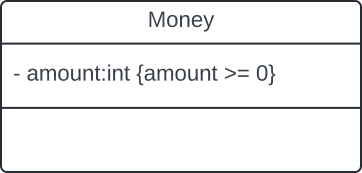
\includegraphics[scale=0.4]{part two/Objektorientierte Analyse/img/moneyocl}
    \caption{Die OCL-Notation in Verbindung mit einem UML-Klassendiagramm zur Spezifizierung des Wertebereichs des Attributes \textit{amount}. (Quelle: eigene)}
    \label{fig:moneyocl}
\end{figure}
\section{Beziehungen von Klassen}

Klassen können auf drei unterschiedliche Arten miteinander in Beziehung stehen:

\begin{itemize}
    \item \textbf{Abhängigkeit} \textit{Dependency}
    \item \textbf{Assoziation} \textit{Association}
    \item \textbf{Vererbung} \textit{Inheritance}
\end{itemize}

\noindent
Bei der Analyse müssen diese Arten von Beziehungen ermittelt werden, damit entsprechend modelliert werden kann.\\

\subsection*{Abhängigkeiten}
\textbf{Abhängikeiten} nutzten eine gestrichelte Linie.\\
Abhängigkeiten werden \textit{in der Analyse} i.d.R. selten modelliert.\\
Als Beispiel für eine Abhängigkeit sei eine \textit{Benutzt-Beziehungen} in Form eines \textit{formalen Parameter} gegeben: Der aktuelle Parameter überdauert den Aufruf einer Methode in einer Klasse, für die diese Abhängigkeit modelliert werden soll, nicht.\\
Gleicherweise kann auch eine \textit{lokale Variable} eines bestimmten Typs eine Abhängigkeit bedeuten.

\subsection*{Assoziation}
Unter einer \textbf{Assoziation} versteht man, dass ein Objekt ein anderes Objekt derselben oder anderen Klasse \textit{dauerhaft} kennt.\\
Assoziationen werden anhand einer durchgezogenen Linie dargestellt.\\
Wird in einem Objekt einer bestimmten Klasse in einem Attribute eine Referenz auf ein Objekt einer anderen oder derselben Klasse gespeichert, existiert eine Assoziation zwischen diesen beiden Klassen.

\subsection*{Vererbung}
Eine \textbf{Vererbung} bedeutet in Vererbungsrichtung eine \textbf{Spezialisierung}, entgegengesetzt eine \textbf{Generalisierung}\footnote{
bzw. \textit{Verallgemeinerung} im Skript (vgl.~\cite[7]{Wed09b}).
}.

\subsection*{Polymorphie}
Eine weitere Bedeutung der Vererbungsbeziehung, ist, dass eine Instanz einer Klasse genauso verwendet werden kann wie eine Instanz seiner übergeordneten Klasse. Allgemein faßt man dies unter \textbf{Polymorphie} zusammen.\\
Als Konsequenz folgt, dass immer dann, wenn ein bestimmter Typ gefordert wird, auch sein Untertyp erlaubt ist (vgl.~\cite[466]{Ull23}), was der Kern des \textit{Liskovschen Substitutionsprinzips}\footnote{
    ``Wikipedia - Liskov substitution principle``: \url{https://en.wikipedia.org/wiki/Liskov_substitution_principle}, abgerufen 11.04.2024
} ist\footnote{
    s.a. ``Wikipedia - Covariance and Contravariance``: \url{https://en.wikipedia.org/wiki/Covariance_and_contravariance_(computer_science)}, , abgerufen 11.04.2024
}.\\

\input{part two/Objektorientierte Analyse/domänenmodell}
\section{Modellierung der Dynamik}

\noindent
In der \textbf{statischen Modellierung} im Domänenmodell werden Klassen in ihrem \textit{Zusammenhang} modelliert.\\

\noindent
Das statische Modell gibt keine Informationen über den Zustand eines Objektes oder wie Botschaften untereinander ausgetauscht werden, und wie sich Objekte / Klassen daraufhin verhalten.\\

\noindent
Um darzustellen, wie sich Klassen oder Objekte verhalten, nutzt man das \textbf{dynamische Modell}.\\

\noindent
Hierzu werden in der \textbf{Analyse} Zustände und Zustandsübergänge eines Systems sowie Aktivitäten modelliert.\\
Grundlage sind Dokumente der Anforderungen, die \textbf{Verhalten} beschreiben, also\textbf{User Stories}, \textbf{Anwendungsfälle} und \textbf{Szenarien}.\\
Die dort beschriebenen Abläufe werden bei der dynamischen Modellierung konkretisiert und genauer definiert.

\subsection*{Zustände und Zustandsänderungen}
\textbf{Systeme} (\textit{Klassen}, \textit{Subsysteme}, \textit{Anwendungen}) können \textbf{Zustände} besitzen, die sich verändern können.\\

\noindent
Oft sind nur Übergänge zwischen bestimmten Zuständen möglich.\\

\noindent
Die grafische Darstellung dieses Verhaltens erreicht man über \textbf{UML-Zustandsdiagramme} (s. Abbildung~\ref{fig:statediagram}).

\begin{figure}
    \centering
    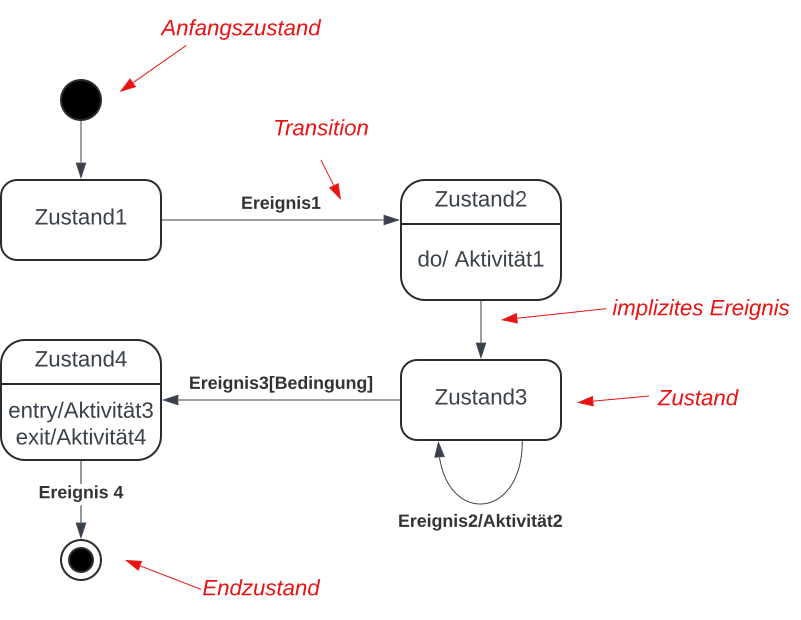
\includegraphics[scale=0.4]{part two/Objektorientierte Analyse/img/statediagram}
    \caption{In der Objektorientierung werden Zustandsautomaten mit Hilfe von Zustandsdiagrammen (\textit{statechart diagram}) dargestellt. Die in der Abbildung gezeigten /do/entry/exit-Aktivitäten werden innerhalb eines Zustands aufgerufen. Ein \textit{implizites Ereignis} (auch: \textit{Beendigungsereignis}) liegt vor, wenn die mit dem Vorgängerzustand verbundene Verarbeitung beendet ist, und eine \textit{Transition} in den Folgezustand führt. (Quelle: in Anlehnung an~\cite[90, Abb. 2.11-6]{Bal05})}
    \label{fig:statediagram}
\end{figure}

\subsection*{Aktivitätsdiagramme}
Bei Zustandsdiagrammen erschließt sich der Ablauf von Aktivitäten meist nur indirekt, da bspw. keine Auskunft über die beteiligten Akteure modelliert werden können.\\

\noindent
Aus diesem Grund verwendet man \textbf{UML-Aktivitätsdiagramm}, in denen Aktivitäten in ihrer möglichen Abfolge und ihrer Zuordnung zu Akteuren modelliert werden.\\

\noindent
Darüberhinaus kann mit Aktivitätsdiagrammen  auch der Fluss von Informationen un die Auswirkung auf Objekte dargestellt werden.\\

\vspace{2mm}
\begin{tcolorbox}
Aktivitätsdiagramme sind zur Modellierung von User Storys, Szenarien oder Anwendungsfällen geeignet.
\end{tcolorbox}
\vspace{2mm}
\section{Analysemuster}\label{sec:analysemuster}

\subsection*{Muster}
Im Software Engineering versteht man unter dem Begriff \textit{Muster} (\textit{Pattern}) \textbf{vorgefertigte Lösungsschablonen für verallgemeinerte Probleme}.\\

\noindent
Bei der Entwicklung tauchen häufig ähnliche Probleme auf, bei denen sich auch die Art der Lösung entsprechend ähnelt.\\

\noindent
Die Beschreibung der verallgemeinerten Probleme und Lösungen auf eine \textbf{formalisierte Weise} nennt man \textbf{Muster}.\\

\noindent
Muster müssen zur Anwendung auf ein konkretes Problem \textit{konkretisiert} werden.\\

\noindent
Im Bereich des Software Engineerings gibt es Muster für \textbf{Analyse}, \textbf{Architektur}, \textbf{Entwurf}.

\subsection*{Vorteile}

\begin{itemize}
    \item es stehen \textbf{bewährte Standardlösungen} zur Verfügung
    \item Verwendung bereits bewährter Lösungen ist oft \textbf{schneller und besser} als selbstentwickelte neue Lösungen
    \item Muster helfen bei der \textbf{Kommunikation}
\end{itemize}


\subsection*{Standardisierte Beschreibung}

\begin{itemize}
    \item Beschreibung des Problems in seinem Kontext
    \item Lösung
    \item Beispiele
    \item Gegebenenfalls Antimuster
\end{itemize}

\noindent
Eine Auswahl wichtigster Analysemuster in der o.a standardisierten Beschreibung findet sich in~\cite[22 ff.]{Wed09b} und wird im Folgenden verkürzt wiedergegeben.

\subsection{Exemplartyp (Abstraction - Occurence)}

\subsubsection*{Problem}
\begin{itemize}
    \item Objekte einer Klasse ähneln sich untereinander und tragen gemeinsamen, gleiche Informationen oder besitzen gleiches  Verhalten, unterscheiden sich aber wesentlich
    \item dieser Zusammenhang zwischen den Klassen soll zum Ausdruck gebracht werden
    \item es soll vermieden werden, dass mehrere Instanzen identische Daten mehrfach beinhalten
\end{itemize}

\subsubsection*{Lösung}
\begin{itemize}
    \item Gemeinsame Daten beinhalten Objekte der Klasse \code{Abstraction}
    \item individuelle Daten beinhalten Objekte der Klasse \code{Occurence}
\end{itemize}

\subsubsection*{Beispiel}
s. Abbildung~\ref{fig:abstractionoccurence}

\begin{figure}
    \centering
    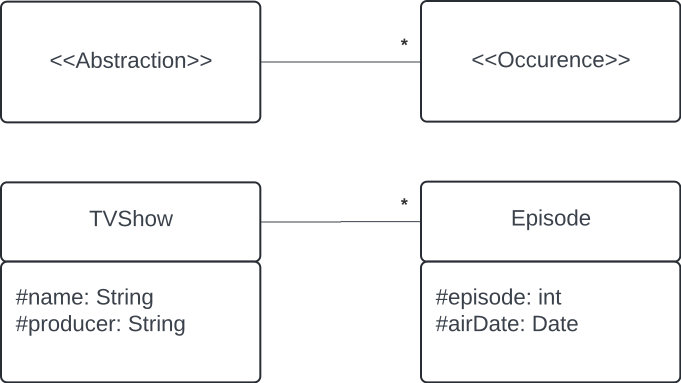
\includegraphics[scale=0.4]{part two/Objektorientierte Analyse/img/abstractionoccurence}
    \caption{Beispiel für das \textit{Abstraction-Occurence-Pattern}. (Quelle: eigene)}
    \label{fig:abstractionoccurence}
\end{figure}


\subsubsection*{Antipattern}
\begin{itemize}
    \item Alle Daten als Attribute einer Klasse modellieren (Zusammenhang von Klassen mit gleichen Daten wird nicht ausgedrückt)
    \item Vererbung (jedes Exemplar eine eigene Klasse)
\end{itemize}


\subsubsection*{Grenzen}
Kann nur sinnvoll eingesetzt werden, wenn die einzelnen Exemplare sinvoll unterschieden werden können, bspw. anhand einer \textbf{Identity}.



\subsection{Wechselnde Rollen (Player - Role)}

\subsubsection*{Problem}
\begin{itemize}
    \item ein Objekt kann in unterschiedlichen Kontexten verschiedene Verantwortlichkeiten und Beziehungen haben
    \item die Verantwortlichkeiten können sich ändern
\end{itemize}

\subsubsection*{Lösung}
\begin{itemize}
    \item Verantwortlichkeiten aus dem Objekt (\code{Player}) nehmen
    \item Verantwortlichkeiten in Objekte (\code{Role}) auslagern
    \item Konkrete Rollen erben von einer Rollensuperklasse
\end{itemize}

\subsubsection*{Beispiel}
s. Abbildung~\ref{fig:playerrole}

\begin{figure}
    \centering
    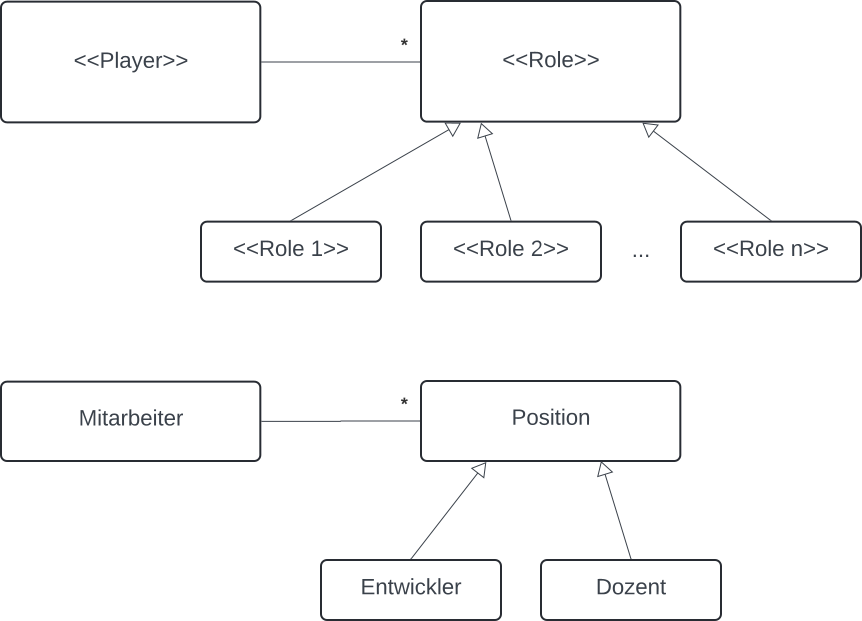
\includegraphics[scale=0.4]{part two/Objektorientierte Analyse/img/playerrole}
    \caption{Beispiel für das \textit{Player-Role-Pattern}. (Quelle: eigene)}
    \label{fig:playerrole}
\end{figure}


\subsubsection*{Antipattern}
\begin{itemize}
    \item Vererbung (eine Klasse identifiziert sich über den Typ der Rolle)
\end{itemize}


\subsection{Allgemeine Hierarchie (General Hierarchy, Kompositum)}

\subsubsection*{Problem}
\begin{itemize}
    \item Objekte können hierarchisch angeordnet sein
    \item Jedes Objekt kann maximal einem Objekt untergeordnet sein
    \item manche Objekte dieser Hierarchie können keine untergeordneten Objekte haben
\end{itemize}

\subsubsection*{Lösung}
\begin{itemize}
    \item Klassen werden von einer Superklasse \code{Node} abgeleitet
    \item Klassen, die andere Klassen referenzieren können, sog. \code{SuperiorNode}s, besitzen Referenzen auf \code{Node}s
    \item Klassen, die keine anderen Klassen referenzieren können, sind \code{NonSuperiorNodes}s
\end{itemize}

\subsubsection*{Beispiel}
s. Abbildung~\ref{fig:generalhierarchy}

\begin{figure}
    \centering
    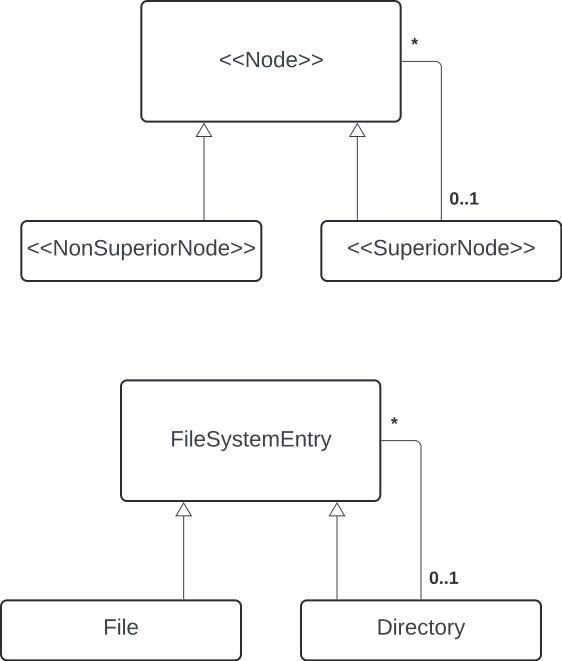
\includegraphics[scale=0.4]{part two/Objektorientierte Analyse/img/generalhierarchy}
    \caption{Beispiel für das \textit{General-Hierarchy-Pattern}. (Quelle: eigene)}
    \label{fig:generalhierarchy}
\end{figure}


\subsubsection*{Antipattern}
\begin{itemize}
    \item Vererbung: Die Vererbung beschreibt \textit{kann-verwendet-werden-als} oder auch \textit{ist-ein}, was bei einem Kompositum aber nicht immer zutrifft.
\end{itemize}


\begin{tcolorbox}
    \blockquote[{\cite[28, Hervorhebung eigene]{Wed09b}}]{
        Beim Muster \textit{Allgemeine Hierarchie} wird die Hierarchie von Objekten modelliert, nicht die Hierarchie von Klassen.
    }
\end{tcolorbox}



\section{Dialogentwurf}
Im \textbf{Dialogentwurf} wird die Schnittstelle zwischen Anwendern und einem System entworfen, die sogenannte \textbf{Benutzeroberfläche}.\\

\noindent
Dabei wird geplant

\begin{itemize}
    \item welche Informationen an welcher Stelle angezeigt werden
    \item welche Aktionen in welchem Zusammenhang ausgeführt werden können
    \item wie die Abläufe für die Benutzer(gruppen) sein werden
    \item wie die graphische Oberfläche gestaltet wird
\end{itemize}

\noindent
Der Dialogentwurf ist wichtig für den Erfolg einer Software: Der Dialog ist das \textit{Gesicht der Anwendung} und deswegen oft entscheidend für die Zufriedenheit der Endnutzer und den Kauf des Produktes.\\

\noindent
Technische Randbedingungen und kommerzielle Interessen müssen bei dem Dialogentwurf berücksichtigt werden.


\subsection{Vorgehen}

Folgendes Vorgehen wird vorgeschlagen (vgl.~\cite[29]{Wed09b}):

\begin{enumerate}
    \item Entscheiden, um welche prinzipielle Art der Anwendung es sich handelt
    \item \textbf{Informationsarchitektur} planen: Inhalte und Verteilung der Inhalte überlegen
    \item basierend auf diesen Überlegungen wird die äußere Struktur und das äußere Erscheinungsbild entworfen
\end{enumerate}

\noindent
Grundlage für diese Arbeiten sind die \textbf{Anforderungen} und die bisherigen \textbf{Ergebnisse der Analyse}.

\subsubsection*{Informationsarchitektur}
Die \textbf{Informationsarchitektur} (\textbf{logische Gestalt}) einer Anwendung definiert, wie die Informationen und die Funktionalität einer Anwendung strukturiert sind, ohne bereits einen konkreten graphischen Entwurf vor Augen zu haben (vgl.\cite[30]{Wed09b}).\\

\noindent
Die Informationsarchitektur definiert außerdem die \textbf{Navigation} für die Benutzer.\\

\noindent
Es wird unterschieden zwischen \textbf{Primärdialogen} und \textbf{Sekundärdialogen}:

\begin{itemize}
    \item \textbf{Primärdialoge}: Stehen dem Benutzer zur Aufgabenerledigung zur Verfügung
    \item \textbf{Sekundärdialoge}: Führen Hilfsarbeitsschritte durch
\end{itemize}

\subsubsection*{Objektorientiertes und Anwendungsfallorientiertes Bedienkonzept}
Bei den Bedienkonzepten unterscheidet man zwischen \textbf{objektorientiertem}\footnote{
\textit{objektorientiert} nicht im Sinne von OOP
} und \textbf{Anwendungsfallorientiertem} Bedienkonzept:

\begin{itemize}
    \item \textbf{Objektorientiert}: Auf in der Oberfläche ausgewählte Objekte können Aktionen durchgeführt werden.
    \item[] Bei dem Entwurf kann man sich am Domänenmodell orientieren, als Faustregel gilt: Jede Domänenklasse benötigt einen Dialog zur Ansicht, Neuanlage und Änderung, für jede $1:n$-Assoziation wird ein Listendialog benötigt
    \item \textbf{Anwendungsfallorientiert}: Je Anwendungsfall gibt es einen Dialog\footnote{
    Dialog ``Adresse ändern``, ``Benutzerkonto einsehen`` \ldots
    }.
\end{itemize}


\subsubsection*{Dialogablaufplan}
Einzelne Dialoge werden als Rechtecke dargestellt und mit ihren Titeln versehen.\\
Übergänge zwischen den Dialogen werden als Pfeile dargestellt.\\
In einem separaten Dokument kann für jeden Dialog der INhalt festgehalten werden (in tabellarischer Form also Eingabefelder, mögliche Aktionen...).

\subsubsection*{Physische Form}
Neben der \textbf{logischen} ist auch die \textbf{äußere Gestalt} zu entwerfen, die \textbf{physische Form}.\\
Hierbei wird u.a. entschieden, ob die Anwendung aus einem komplexen Fenster besteht, in dem sich Teile ändern (die einzelnen Kacheln, \textit{Tiles}, wie bspw. in einem Email-Programm), ob sich der INhalt des Fensters ändert (bspw. \textit{Wizards}), oder ob es mehrere Fenster geben soll.\\
I.d.R. sind bei großen Anwendungen Mischlösungen anzutreffen, wo bspw. der \textbf{Primärdialog} in einem gekachelten Fenster implementiert ist und \textbf{Sekundärdialoge} in anderen Fenstern.\\

\noindent
Anschließend kann der genaue Inhalt und das graphische Aussehen bestimmt werden.

\subsubsection*{Prototyping}
Das \textbf{Prototyping} kann bspw. über Mockups bzw. Wireframes realisiert werden, oder auc mit Bleistift und Papier.\\
In jedem Fall sind so Änderungswünsche in einem Kundengespräch schnell und unkompliziert durchgeführt.

\subsection{Ergonomie}
Mit dem Begriff \textbf{Software-Ergonomie} (\textit{Usability}) wird die \textbf{Benutzbarkeit} bzw. \textbf{Gebrauchstauglichkeit} von Software bezeichnet.\\

\noindent
Die Ergonomie ist wichtig, damit

\begin{itemize}
    \item die Anwendung von den Benutzern akzeptiert wird
    \item die Benutzer längere Zeit ohne phsysische und psychische Ermüdungserscheinungen arbeiten können\footnote{
    in Deutschland bspw. geregelt über die \textit{Bildschirmarbeitsverordnung}, wenn Softwrae für kommerzielle Zwecke eingesetzt wird.
    }
\end{itemize}

\noindent
In Sicherheitskritischen Bereichen wie der Luftfahrt ist Ergonomie wichtig, da Ermüdungserscheinungen fatale Folgen haben können.\\

\noindent
Das Ziel der \textbf{User Experience} (\textbf{UX}, \textit{Nutzungserlebnis}) ist ein möglichst angenehmes Nutzungserlebnis, was nicht unbedingt mit einer guten Ergonomie verbunden ist.\\

\noindent
Einflüsse auf die Ergonomie haben u.a. die logische Aufteilung der Inhalte, die graphische Gestaltung und die Benutzerführung.

\subsubsection*{Graphische Gestaltung}
Die \textbf{graphische Gestaltung} ist für die Ergonomie einer Software nicht nur für das Erleben, sondern auch für eine stressfreie Nutzung wichtig.\\

\noindent
Als Grundregeln gelten hier die übersichtliche Gestaltung der Benutzeroberfläche, indem

\begin{itemize}
    \item genügend Platz gelassen
    \item Zusammengehöriges gruppiert und voneinander abgesetzt wird
    \item nicht zuviele verschieden Schriftarten verwendet werden
    \item Farben sparsam und konsistent ohne zu große Kontraste eingesetzt werden
    \item Farben und Schriftarten auf die Bedürfnisse der Nutzer anpassbar sind
\end{itemize}

\subsubsection*{Styleguide}
Gleiche Elemente einer Benutzeroberfläche sollten gleich aussehen und nach einer durchgängigen Logik angeordnet sein.\\
Solche Richtlinien lassen sich in einem \textbf{Styleguide} zusammenfassen.

\subsubsection*{DIN EN ISO 9241}
Die für die \textbf{Ergonomie von Bildschirmarbeitsplätzen} wichtigste Norm ist die \textbf{DIN EN ISO 9241}\footnote{
s. \url{https://de.wikipedia.org/wiki/ISO_9241}, abgerufen 13.04.2024
} (\textit{Ergonomie der Mensch-System-Interaktion}).\\
Für die Gestaltung von Benutzeroberflächen ist insb. Teil 110 \textit{Grundsätze der Dialoggestaltung} relevant, in der 7 Gestaltungsgrundsätze zusammengefasst sind:

\begin{itemize}
    \item \textbf{Aufgabenangemessenheit}: Ein Dialog ist den Aufgaben angemessen, wenn er die Benutzer unterstützt, die Aufgaben effektiv und effizient zu erledigen.
    \item \textbf{Selbstbeschreibungsfähigkeit}: Für die Benutzer ist jederzeit offensichtlich, im welchem Dialog und an welcher Stelle im Dialog sie sich befinden, welche Handlungen unternommen werden und wie diese ausgeführt werden können.
    \item \textbf{Steuerbarkeit}: Der Benutzer ist in der lage, den Dialogablauf zu starten und seine Richtung und Geschwindigkeit zu ändern, bis das Ziel erreicht ist (bspw. Rückgängigmachfunktion, Vor-/Zurück-Buttons \ldots).
    \item \textbf{Erwartungskonformität}: Ein Dialog ist erwartungskonform, wenn er konsistent ist und den Merkmalen des Benutzers entspricht (Kenntnisse Arbeitsgebiet, Ausbildung, Erfahrung, allgemein anerkannter Konventionen, bspw. einheitliche Verwendung von Funktionscodes und Funktionstasten in allen Dialogen).
    \item \textbf{Fehlertoleranz}: Das beabsichtigten Arbeitsergebnis wird trotz erkennbar fehlerhafter Eingaben mit keinem oder \textbf{minimalen Korrekturaufwand} seitens des Benutzers erreicht.
    \item \textbf{Individualisierbarkeit}: Das Dialogsystem erlaubt Anpassungen an Erfordernisse der Arbeitsaufgabe sowie individuelle Fähigkeiten und Vorlieben des Benutzers.
    \item \textbf{Lernförderlichkeit}: Der Benutzer wird beim Erlernen des Dialogs unterstützt und angeleitet.
\end{itemize}

\subsubsection*{Barrierefreiheit}
Unter Barrierefreiheit \textit{Accessibility} versteht man, dass eine Software so gestaltet ist, dass auch Menschen mit Behinderungen mit dieser Software arbeiten können.

\section{Zusammenfassung}

\begin{itemize}
    \item Anforderungen lassen sich bei Projekten vorab nicht genügend festlegen.
    \item Fehlt im Team die Erfahrung oder werden neue Technologien eingesetzt, ist ein ausgereifter Entwurf nicht machbar.
    \item Bei großen Projekten würde man unter diesen Voraussetzungen mit dem Wasserfallmodell nicht flexibel genug sein,
    um auf Änderungen reagieren zu können.
    \item Aus diesem Grund gibt es alternative Modelle, die eingesetzt werden können:
        \begin{itemize}
            \item \textbf{inkrementell}: Aufteilung der Anforderungen, so dass Teilsysteme umgesetzt und an den Kunden ausgeliefert werden können
            Die Teilsysteme werden sequentiell bearbeitet.
            \item \textbf{iterativ}: In Iterationen wird das Projekt in Zeitabschnitte unterteilt, in denen die Anforderungen umgesetzt werden; entsprechend dem Spiralmodell zunächst die risikoreichsten.
            Vorhergehende Ergebnisse werden in darauffolgenden Iterationen weiterbearbeitet.
            Ein bekanntes iteratives Modell ist \textit{RUP}, bei dem einzelne Phasen Ergebnis-Artefakte liefern, wie Anwendungsfälle oder Klassendiagramme.
            \item \textbf{nebenläufig}: Die Aufgaben werden aufgeteilt in parallel (oder nacheinander) bearbeitbare Aufgaben, die dann von den Mitarbeitern umgesetzt werden.
        \end{itemize}
    \item Die genannten Modelle werden häufig nicht isoliert betrachtet, sondern je nach Projekt auch kombiniert, insb. bei dem \textbf{agilen Vorgehen}.
\end{itemize}
\newpage

